\chapter{Cylindrical Algebraic Decomposition}

\[
	\exists x, x^2+bx+1\leq 0 \iff (b\leq -2) \lor (b \geq 2)
\]

CAD for $f(x) = x^2 + bx + 1$:

\begin{figure}[h]
	\centering
	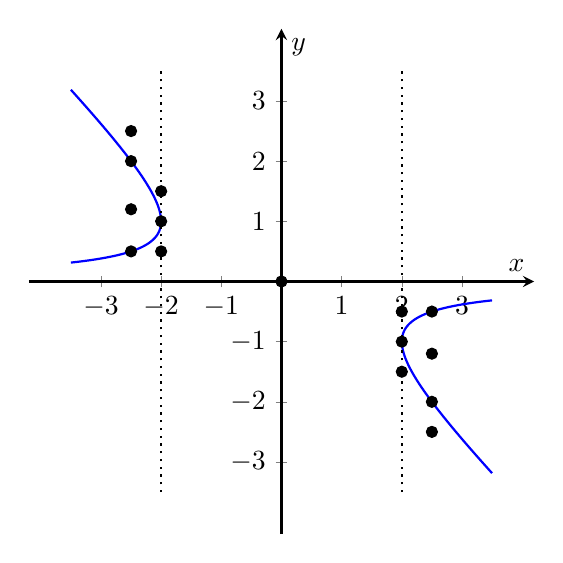
\begin{tikzpicture}
		\begin{axis}[
				axis lines=middle,
				axis line style={thick},
				xmin=-3.5, xmax=3.5,
				ymin=-3.5, ymax=3.5,
				xtick={-3,-2,-1,0,1,2,3},
				ytick={-3,-2,-1,0,1,2,3},
				width=8cm,    % Adjusted size to fit on one page
				height=8cm,
				xlabel={$x$},
				ylabel={$y$},
				enlargelimits,
				grid=none,
				samples=100,
				domain=-3.5:3.5,
			]

			% First curve
			\addplot [
				blue, thick,
				domain=-3.5:-2.0001,
				samples=100
			] {0.5 * (sqrt(x^2 - 4) - x)};

			\addplot [
				blue, thick,
				domain=2.0001:3.5,
				samples=100
			] {0.5 * (sqrt(x^2 - 4) - x)};

			% Second curve
			\addplot [
				blue, thick,
				domain=-3.5:-2.0001,
				samples=100
			] {0.5 * (-sqrt(x^2 - 4) - x)};

			\addplot [
				blue, thick,
				domain=2.0001:3.5,
				samples=100
			] {0.5 * (-sqrt(x^2 - 4) - x)};

			% Dotted vertical gridlines at x = ±2
			\draw[dotted, thick] (axis cs:2,-3.5) -- (axis cs:2,3.5);
			\draw[dotted, thick] (axis cs:-2,-3.5) -- (axis cs:-2,3.5);

			% Black points
			\addplot[
				only marks,
				mark=*,
				black,
				mark size=2pt
			] coordinates {
					(-2, 1.5) (-2, 1) (-2, 0.5)
					(-2.5, 0.5) (-2.5, 1.2) (-2.5, 2) (-2.5, 2.5)
					(0, 0)
					(2, -1.5) (2, -1) (2, -0.5)
					(2.5, -0.5) (2.5, -1.2) (2.5, -2) (2.5, -2.5)
				};

		\end{axis}
	\end{tikzpicture}
	\caption{Illustrating the cells and the samples.}
	\label{fig:curve_plot}
\end{figure}

Project the valid cells onto the $b$-axis and take the disjunction of the intervals.
